\chapter{Related Work} \label{ch:related}

\section{Related Work}

\subsection{Dataflow Streaming Engines}

In contrast to the standalone Timely Dataflow library, many state-of-the-art
dataflow streaming engines have been designed and engineered from the start
to run multiple concurrent dataflow computations in a cluster. One of the
goals of this thesis was to provide such functionality for Timely Dataflow
based programs. Thus, in this section, we will mainly focus on the execution
and management aspect running multiple concurrent dataflow computations. Less focus is
put on the differences in the programming and synchronization model these 
other systems provide. Our system currently also does not provide any fault
tolerance guarantees. This is also a notable difference our system has compared
to related work, which often put heavy emphasis on providing strong fault
tolerance.

\subsubsection{Spark Streaming}

Spark Streaming \cite{sparkstreaming} is a streaming engine based on the Spark
cluster computation framework. Spark Streaming executes streaming dataflow
computations by turning them into stateless, fault-tolerant batch computations.
These batches are submitted as tasks to the underlying Spark engine. \cite{spark} 

\paragraph{Process Model}

In Spark, computational tasks work is modeled as transformations on partitioned
collections of records called \emph{resilient distribute datasets}. The
runtime schedules the execution of the transformations on a distributed set of
worker nodes. By tracking the lineage of transformations, Spark is able to
recover computations by reissuing lost transformations. Based on the model,
Spark Streaming models stateful, conceptually continuous dataflow computations
as small stateless microbatches. This model of execution is very different from
Timely's continuous operator model. In Timely, both the operator scheduling
and the data of the computation are managed directly by the workers themselves,
which are hosted by long living operating system processes. In Spark however,
the data and code is managed by the system. Because of this, Spark is not only
able to provide strong fault tolerance by reissuing failed computations, Spark
is also able to load balance concurrently running streams and mitigate stranglers.
While we currently do not offer these features, Timely does achieve much lower
latencies than Spark Streaming, which is mostly enabled by the fact that every
Timely worker manages itself independently.

%TODO driver processs

\subsubsection{Storm \& Heron}

Heron \cite{heron} is the API-compatible successor of the Storm \cite{storm}
streaming dataflow engine.
Both Storm and Heron call their dataflow computations \emph{topologies}, which 
are directed acyclic graphs of spouts (stream sources) and bolts
(stream transformers). Parallelism is achieved by the user specifying the
number of instances for each bolt and spout, as well as the partitioning
strategy between them.

\paragraph{Process Model}

The process model of Storm is very similar to our approach: A topology
(roughly corresponding to a query in our system) is executed by multiple
\emph{worker processes}. These are operating system processes which are distributed
over different machines, thus similar to our query processes. Every machine hosts
a \emph{supervisor}, which not only monitors the local worker processes, but also spawns new worker
processes on behalf of the \emph{Nimbus}, making Storm's supervisors similar to our executors.
The Nimbus is a central process to which new topologies are submitted, mirroring our coordinator.

Heron mostly differs from Storm in its internal architecture. Most notably, in
Heron every spout or bolt now runs in its own operating system process. All processes
belonging to the same topology are grouped together in an operating system container.
The motivation for this change are reported to be better debug-ability
and simpler resource management. The authors also state that their topologies
seldom have more than three stages (i.e. bolts/spouts). We believe that such
an architecture would not make much sense for Timely, as its operators are typically
more numerous and more lightweight.

Another major change from Storm's architecture
is the fact Heron does not have a central coordinating process anymore. Being
a single point of failure and a bottleneck, the Nimbus was considered to be a
flawed design. Heron thus replaces the old responsibilities of the Nimbus by
offloading them into a small set of independent processes. This might be something
to consider for futures extensions to our coordinator.

\subsubsection{Flink}

Flink \cite{flink} is a dataflow streaming engine for directed acyclic
dataflow graphs, however it does have support for iterative dataflows on the
outermost level. Flink interleaves control events with data records. Control
events are used for progress tracking and fault tolerance, which is done through
snapshots. Progress tracking is implemented with global \emph{low watermarks}, which
denote the minimum timestamp which can be emitted at the sources of the
topology, enabling Flink to perform out-of-order processing.

\paragraph{Process Model}

The runtime architecture of Flink also uses a central process called the
\emph{job manager}, which accepts and manages computations submitted by
the client. The job manager takes the user submitted code, translates it into
an execution plan and potentially optimizes it.

The computations themselves are executed inside worker processes called
\emph{task managers}. Task managers provide a similar function as our executors, in that
they provide access to computational resources and are distributed over
potentially multiple machines. Like our executors, they can be dynamically added and announce themselves at the
job manager. However, in contrast to our executors, task managers directly execute the
operators and manage any data exchange between them. In our system, this task is done by the
query library in conjunction with the Timely runtime.

For resource management purposes, each task manager provides
a predefined number of task slots. These typically correspond with the number of CPU cores,
though it is not enforced that a slot only uses one thread. The available memory is also distributed
equally between the task slots of a task manager. The submitted dataflow computation is split up
in multiple subtasks (one subtask typically corresponding to one operator), and each subtask is assigned
to a task slot. Subtasks from the same submission can share a task slot
if the operator supports it. This is used for example for pipelined operators which don't
require any exchange of data with operators running in other task slots.
Because task managers can have multiple task slots, they can run operators from different
computations within the same operating system process, similar to Spark Streaming.
Unlike Spark Streaming however, these operators are continuous and
do not migrate to other task slots during normal operation.

\subsection{Sharing Dataflow Streams}

In this section we discuss how composition of different dataflow streams 
can be achieved in other systems.

\subsubsection{Kafka}

Kafka \cite{kafka} is a distributed platform for accumulating and sharing streams. It provides
a topic-based publish/subscribe service, where topics can have multiple partitions. Producers append
their data to one or more partition, allowing subscribers to read from it.
The data within a partition is stored persistently, allowing subscribers to
read all previously published data sequentially and continue where they left
of in case of failures. The data within a partition is ordered, however there
is no defined ordering across multiple partitions of the same topic. Recent
versions of Kafka also supports the assignment of event timestamps to messages.

\paragraph{Integration with Dataflow Engines}

Both Spark Streaming and Flink provide official connectors for Kafka, allowing
dataflow computations to stream data from or to Kafka topics. Flink additionally supports
the extraction of timestamps from topics. Similar to our system, Flink also provides a
mechanism to exact watermarks from Kafka sources, allowing a partition
to contain out-of-order data. Like our system, Flink is able to unify
progress tracking information from multiple sources.

In some ways, Kafka is very similar to our publish/subscribe as we also expose
potentially partitioned streams from which consumers, such as dataflow programs,
can subscribe to. In contrast to Kafka, we have a strict one-to-one mapping between stream
partitions and topics. Stream partitions in our system are only grouped together
by naming conventions on the topics.
 
Another difference between Kafka and our system is that Kafka's subscribers are
\emph{pulling} data from their source, whereas in our system data is \emph{pushed}
from the source to the subscribers. This implies that in our system the publisher
does not know about the progress of the subscriber, which can lead
to backpressure issues if the subscribers are slow.

\paragraph{Kafka Streams}
In additions to the above mentioned adapters, Kafka also provides its own
streaming engine called Kafka Streams. It provides a simple acyclic dataflow
model which uses Kafka topics as sources and sinks, thus acting as transformers.
Parallelism is achieved by instantiating the dataflow graph on multiple threads.
Partitioning of the data happens before it is fed to the individual instances
of the dataflow graph.

Like standalone Timely Dataflow, Kafka Streams is implemented as a library. It
is left to the user to deploy and launch instances of the streaming computation.

\subsubsection{MillWheel}

MillWheel \cite{millwheel} is a stream processing framework used to implement
the dataflow model proposed by Google \cite{google}. MillWheel conceptually
treats the whole system as a single dynamic dataflow graph: The nodes of the
dataflow graph are user submitted computations (i.e. operators) that are
invoked by the system on receipt of incoming data. Edges are created by the
user specifying which streams a computation consumes and produces. Streams
have uniquely assigned names.

This makes MillWheel essentially a publish/subscribe system, as every individual
operator acts as a subscriber and as a publisher. This is slightly different from
our system and other combinations of dataflow systems that use an external
publish/subscribe mechanism: Streams between operators in our system are anonymous until
explicitly published. In MillWheel however all streams used to connect operators
are automatically made available for subscription by third parties.

Another difference to our approach is the fact that MillWheel lets subscriber
specify how a stream should be partitioned before it is delivered to the consumer.
Aggregation and partitioning is done according to keys, i.e. records with the
same key are always delivered to the same computation instance. Different
computations can however use different keys on the same streams, as every computation
needs to provide a key extraction function for each of its input streams.

Computations run on one or more processes distributed over a dynamic set of
machines. The assignment of computations to machines and keys to computations
is managed by the system itself. Because the system manages persistent state
on behalf of the computations, computations for a certain key can be moved
for load-balancing or restarted in the case of failures.

\cleardoublepage
\chapter{Future Work \& Conclusions} \label{ch:future}

\section{Future Work}

\subsection{Extracting the Dataflow Graph from Queries}

Our system currently treats queries for the most part as black boxes. While we
do dynamically track some information about the query, such as its publications
and subscriptions, the system does not know anything about a queries internal
dataflow graph. The reason for this is discussed in Section \fullref{sec:runtime-graph}:
Timely itself only assembles a type-erased representation of the dataflow graph
during execution. The integrated logging framework also only exposes the
structure of the dataflow graph, but not any properties about the nodes and
edges themselves besides the name of the operators. While further instrumentation
of Timely would certainly be able to provide more insight into the dataflow
graph, solely run-time oriented approaches are limited in what they can do:
Rust does not provide any run-time reflection of types besides unique type
identifiers, and most operators accept user-defined functions to implement
parts of their logic. We therefore believe that some form of static analysis
is unavoidable for extracting precise information about the dataflow graph.
Possibles uses for more precise descriptions of the dataflow graph of a query
are described below.

\subsection{Retroactive Tapping of Dataflow Edges}

With the current publish/subscribe mechanism, query authors are required to
anticipate which operator outputs are of possible interest for subscribers. If
a certain output is not explicitly published through a publish operator, there
is no way for other queries to access it. We believe that some mechanism
for retroactively exposing dataflow edges in a running query would be useful.
Possible use-cases include better diagnostics, more flexible query composition,
and potentially also query optimization.

We considered implementing such a feature as part
of this thesis, and the design choice of topics that can be dynamically added
or removed from the catalog was  explicitly made with such a use-case in mind.
However, due to time constraints, we were not able to pursue an implementation.
In the remainder of this section, we will however present some of our
preliminary ideas.

\paragraph{Exposing Stream Handles}

We believe that it would be relatively easy to instrument Timely such
that it exposes its data streams for later use without much run-time
overhead: Timely's stream handle internally maintains a registrar which
is used by succeeding operators to register themselves as consumers.
When data is sent to an operator's output, the data is pushed one by one into the
queues of the consumers that have registered themselves on that output. By collecting and exposing
the registrars of all edges, it would easily be possible to add new consumers
at run-time. An unresolved issue with this approach however is that it would only allow
the inspection of the \textquote{data plane} of a Timely computation. Because
progress tracking information is delivered separately, a way has to be found to
expose this additional information as well.

\paragraph{Processing intercepted streams}

Previous work on monitoring distributed systems such as P2 \cite{p2} and
Pivot Tracing \cite{pivot} has demonstrated powerful interfaces for
processing and querying intercepted streams of running systems.
We believe that a functionality to tap into dataflow edges of running queries would
enable similar possibilities in our system: By publishing tapped
dataflow edges as topics, other queries could be used to monitor, diagnose, or
extend a running dataflow computation.

Furthermore, the overhead of serializing intercepted tuples could be avoided
by extending the system to dynamically load code into running queries. Systems
such as Pivot Tracing are using Java's ability to dynamically load
bytecode into the running programs. For our Rust-based system we envision a
mechanism where queries are attached as dynamic shared objects onto other
running queries.

\paragraph{Work Deduplication}

A detailed representation of a query's dataflow graph, together with the ability
to tap into dataflow edges, could also be used for query optimization. An example
of this is dataflow path deduplication: If a new incoming query performs the same
sequence of operations on the same stream of data as an already existing
query, we would like to deduplicate this work. By exploiting the fact that
topics act as semantic descriptions of streams, the system could automatically
tap into dataflow edges on the outgoing path of a publication in order to
optimize the subscriptions of submitted queries. Such an optimization however
requires that the system is able to compare the semantics of operators,
i.e. it needs to be able to determine if two operators are equivalent. It
would also require a way for the system to remove or insert operators before
executing the query.
An example of such an optimization is shown in Figure~\ref{fig:queryoptimization}.

\begin{figure}[!htb]
  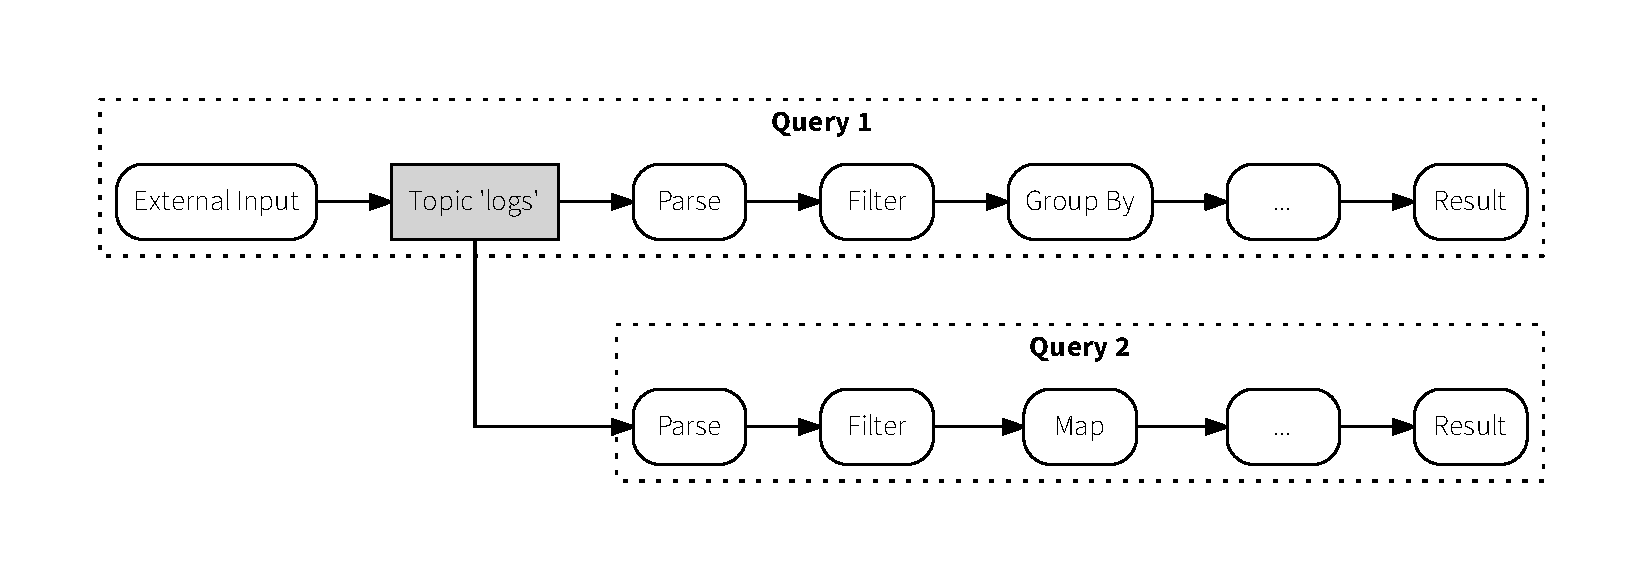
\includegraphics[scale=0.36]{figures/composition/q1q2_man}
  \vspace{-1.5em}
  \begin{center}
  $\Downarrow$
  \end{center}
  \vspace{-1.2em}
  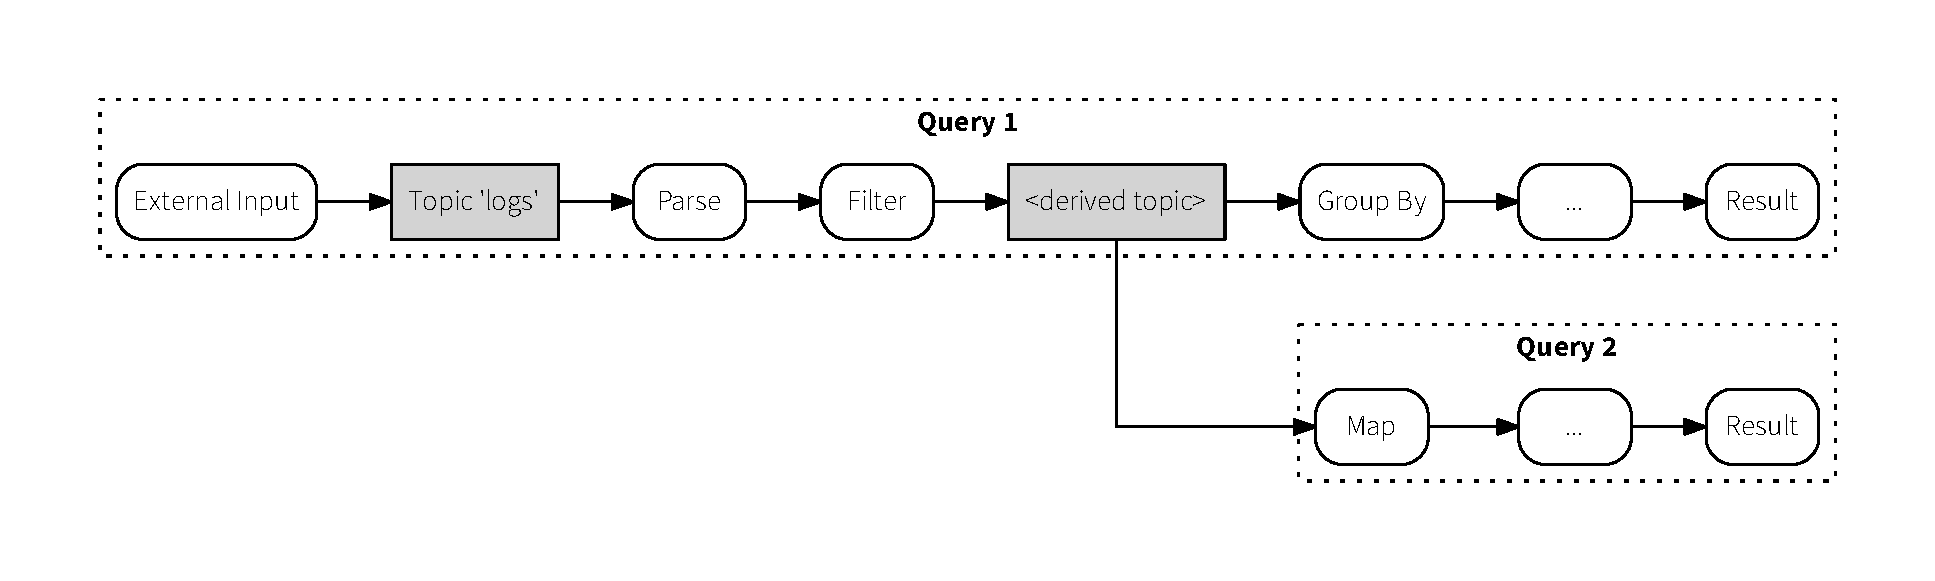
\includegraphics[scale=0.36]{figures/composition/q1q2_auto}
  \caption[Work duplication through derived topics]{
  Work duplication through derived topics. By tapping into dataflow edges
  of the publishing query, the system can optimize the newly arrived
  subscribing query.}
  \label{fig:queryoptimization}
\end{figure}




\subsection{Resource Management}

For the most part, resource management is still an unresolved problem in our
current system. One aspect of this is the placement of queries on the available
executors. It is currently the responsibility of the user to select which executors
will host a new query submission.
The reason for this is that system does not know what conditions have to be
fulfilled in order to execute the query:
The query might access external files or other resources which are currently not
expressed in the system model through the catalog.

However, in many cases automatic placement of queries might be desired. Future
work would have to explore what kind of information a query placement scheduler
requires to perform well, and extending executors or other components to collect
this kind of information.

Another aspect of resource management is resource control. Once a placement
for a query has been selected, the responsible executors might want to ensure
that the available resources are distributed fairly among the
running queries. Currently, CPU and memory usage of queries is solely managed
by the operating system. The use of operating system features such as
Linux \emph{control groups} \cite{cgroups} could be added to more precisely indicate
to the operating system what kind of resources certain queries should have
access to.

Because queries can run arbitrary code and might not be trusted,
future work might also want to investigate sandboxing or other protection
techniques to further isolate queries from each other and the underlying operating
system.

\subsection{Backpressure, Buffering and Persistance}

Our current system does not buffer data at the publisher if there are no
subscribers. It does however buffer outgoing data for connected subscribers
until they consume it or disconnect. This can become an issue if a single
subscriber is slower than the publisher, as its queue will grow and thus
memory consumption increase. Future work has to explore how to throttle
the publishing query in such situations. One possible approach would be the
addition of probes which indicate the subscribers progress. These would then
be used to throttle the input of the publishing query. Previous work \cite{faucet} has
successfully demonstrated the use of such a flow control mechanism within the
scope of a single query, future work would have to explore how to integrate
this with our system.

Tightly coupled queries can already implement such an approach today, as our
system allows two queries to subscribe to each other: Besides the topic published by the producer and
read by the consumer, there would be an additional second topic published by the
consumer and read by the producer used as a back channel for progress probing.

Another approach to deal with slow subscribers could be the introduction of
intermediate buffers, which store the published data in persistent storage. 
This would reduce memory pressure in the presence of slow subscribers and it
would also allow late subscribers to replay the whole data stream, if such
a feature is desired.

Intermediate buffers could also be used to reduce network traffic if many
co-located subscribers consume data from same remote publisher: By having
subscribers read their data from local buffers instead of the remote publisher,
data would only have to be sent once over the network.

\subsection{Partitioning and Filtering by Subscribers}

In our current system, the partitioning scheme of published streams is
determined by the publishers, which either publishes one topic per worker or
a single topic for all workers. If a subscribing query uses a different amount
of workers than there are available topics, the query author of the subscribing
query has to manually distribute these topics among the query's workers.

MillWheel by contrast allows subscribers to provide their own partitioning
functions which are used by the system to automatically decide how data is
routed from the publishers to the subscriber instances. It is not completely
clear how such a functionality could be implemented in our system, as we
currently do not have intermediate message brokers which could do the routing.

One possible implementation approach could however work by allowing subscribers
to tell the publishers about the kind of data they are interested in. Custom
routing functions would then be implemented by the subscribers connecting
to all the publisher partitions, but only receiving a subset of of the published
data based on the provided filters. This approach would be similar to
content-based filtering and routing found in other publish/subscribe systems
\cite{pubsub}.

\clearpage
\section{Conclusions}

\TODO{rewrite}

In this work we have presented a system for deploying Timely Dataflow applications.
In addition to managing the submission of dataflow programs for execution
on a cluster, we also provide facilities for these computations to publish
their streams for consumption by other queries. 

This functionality is used by the
system catalog to expose metadata about the current system state, but more
importantly, it can also be used for query composition.

We demonstrated that query composition can be used to modularize a computation
based on a realistic workload and show that doing so imposes acceptable costs
in terms of memory consumption and execution time overhead.


